\section{实验}
\label{sec:experiments}
\subsection{数据与评价设置}
我们使用CRC和TIGER组织数据。训练集与开发集按空间块划分，支持—查询对以及不同划分之间均保持完整$4\times$输入覆盖范围的分离，并保留患者及切片来源信息。

远端开发队列使用$300$个CRC支持图像块，以及来自$75$张查询切片的$3{,}200$个不同查询图像块，覆盖表~\ref{tab:wsi_tissue}中的11种组织；背景提供有效负类像素。在$11{,}000$个任务中，$7{,}334$个包含目标，$3{,}666$个不含目标。每个任务使用三个正支持点击与两个负支持点击，依据固定规则从支持标注模拟生成，并在各方法间共享。该远端队列用于方法比较与选择。整片评价使用15张切片、152个组织任务。用于整片测试的患者病例均未出现在训练集或开发集中。

\subsection{比较方法与评价指标}
\label{sec:baselines}
我们将FewClick与SANSA、SAM、SAM2、WSI-SAM和SAM-Med2D比较。各方法使用相同的$9{,}500$个新增目标域训练任务、$2{,}375$次更新及支持点击，并使用最终权重进行评价。公开预训练、模型架构、输入视野和适配模块遵循各方法的配置。匹配的量为新增目标域数据适配预算。

SANSA适配其公开Universal adapter，实现支持到查询的传播。SAM系列模型使用由支持信息调节的迁移桥生成自动密集提示；WSI-SAM还使用固定规则生成的稀疏提示。图像编码器均冻结。SANSA使用单个精细视野；SAM、SAM2与SAM-Med2D使用三个对齐视野，WSI-SAM使用精细与$2\times$视野。FewClick与SANSA分别训练7.03M和26.33M个参数。完整的初始化与适配配置见补充材料。

我们报告目标存在查询的类别宏平均Dice，以及目标缺失查询的误报面积比例（FPA）。小目标与大目标分别占有效查询面积的$<20\%$和$\geq20\%$。精确率、召回率以及物理容差为$2\,\mu$m的边界F1用于刻画覆盖与轮廓质量。对于WSI，先在不重复的有效像素上计算每个“切片—目标”组合的Dice，再对各组织内的切片取平均，最后对11种组织等权平均。整片与严格远端评分域遵循第~\ref{sec:wsi}节的定义。

\subsection{同片远端图像块分割}
\begin{table}[t]
\centering
\caption{在11,000个任务上的同片远端分割结果。各任务使用三个正支持点击和两个负支持点击，查询区域无点击。Dice与大目标列分别报告目标存在Dice和大目标Dice。所有指标均为百分比；粗体表示最优值。}
\label{tab:remote}
\small
\setlength{\tabcolsep}{4pt}
\begin{tabular}{@{}lrrr@{}}
\toprule
方法 & Dice $\uparrow$ & 大目标 $\uparrow$ & FPA $\downarrow$ \\
\midrule
SAM & 30.31 & 64.40 & 27.01 \\
SAM2 & 33.60 & 66.50 & 18.91 \\
WSI-SAM & 23.81 & 50.02 & 23.43 \\
SAM-Med2D & 24.28 & 54.80 & 39.87 \\
SANSA & 41.54 & 77.22 & 14.79 \\
FewClick & \textbf{42.11} & \textbf{78.49} & \textbf{7.75} \\
\bottomrule
\end{tabular}
\end{table}

表~\ref{tab:remote}比较了六种方法在相同任务上的表现。FewClick的目标存在宏平均Dice为42.11\%，大目标Dice为78.49\%，目标缺失FPA为7.75\%。SANSA的对应指标分别为41.54\%、77.22\%和14.79\%。FewClick的两项Dice分别提高0.57和1.27个百分点，FPA降低7.04个百分点，相对下降47.6\%。

对75张查询切片进行4,000次配对重采样后，FPA差值的95\%区间为$[-8.37,-5.70]$个百分点，目标存在Dice差值的区间为$[-0.11,1.31]$。FPA区间完全低于零，Dice区间包含零。

\subsection{整片分割}
\begin{table}[t]
\centering
\caption{在15张切片、152个组织任务上的整片类别宏平均Dice（\%）。每个“切片—目标”组合使用一个支持图像块以及三个正点击和两个负点击。严格远端评价排除输入覆盖范围与支持区域相交的相关输出。}
\label{tab:wsi}
\small
\setlength{\tabcolsep}{4pt}
\begin{tabular}{@{}lrr@{}}
\toprule
方法 & 整片 $\uparrow$ & 严格远端 $\uparrow$ \\
\midrule
SAM & 18.86 & 16.63 \\
SAM2 & 23.58 & 21.01 \\
WSI-SAM & 15.85 & 14.25 \\
SAM-Med2D & 13.59 & 11.97 \\
SANSA & 33.23 & 30.12 \\
FewClick & \textbf{43.75} & \textbf{40.98} \\
\bottomrule
\end{tabular}
\end{table}

\begin{table*}[t]
\centering
\caption{六种方法在相同15张WSI上的逐组织整片Dice（\%）。每种组织的得分对有效“切片—目标”组合取平均；$n$为参与该组织评价的切片数。宏平均对11种组织等权计入。粗体表示每行最高的Dice。}
\label{tab:wsi_tissue}
\small
\setlength{\tabcolsep}{0.5pt}
\begin{tabularx}{\textwidth}{@{}p{0.20\textwidth}*{7}{>{\centering\arraybackslash}X}@{}}
\toprule
组织 & $n$ & SAM & SAM2 & WSI-SAM & SAM-Med2D & SANSA & FewClick \\
\midrule
肿瘤上皮 & 15 & 50.02 & 58.79 & 35.53 & 36.87 & 78.97 & \textbf{79.17} \\
肿瘤间质 & 15 & 31.53 & 36.39 & 27.11 & 22.86 & 42.97 & \textbf{55.23} \\
坏死 & 15 & 15.09 & 20.29 & 14.83 & 11.72 & 32.91 & \textbf{44.10} \\
正常腺体 & 15 & 18.35 & 24.27 & 17.41 & 8.77 & 26.10 & \textbf{43.23} \\
正常间质 & 15 & 5.68 & 9.01 & 5.61 & 5.48 & 20.80 & \textbf{25.12} \\
黏膜下层／浆膜 & 15 & 22.75 & 25.18 & 19.94 & 19.47 & 36.15 & \textbf{49.83} \\
肌肉 & 15 & 31.82 & 37.27 & 29.46 & 23.50 & 51.27 & \textbf{61.32} \\
淋巴组织聚集 & 7 & 2.17 & 2.61 & 1.51 & 1.96 & 5.46 & \textbf{34.24} \\
黏液 & 15 & 3.82 & 6.92 & 3.79 & 3.05 & 9.23 & \textbf{18.76} \\
脂肪 & 15 & 22.96 & 30.58 & 16.14 & 13.59 & \textbf{49.51} & 48.67 \\
血液 & 10 & 3.22 & 8.10 & 3.01 & 2.25 & 12.13 & \textbf{21.59} \\
\midrule 宏平均 & -- & 18.86 & 23.58 & 15.85 & 13.59 & 33.23 & \textbf{43.75} \\
\bottomrule
\end{tabularx}
\end{table*}

\begin{figure*}[t]
\centering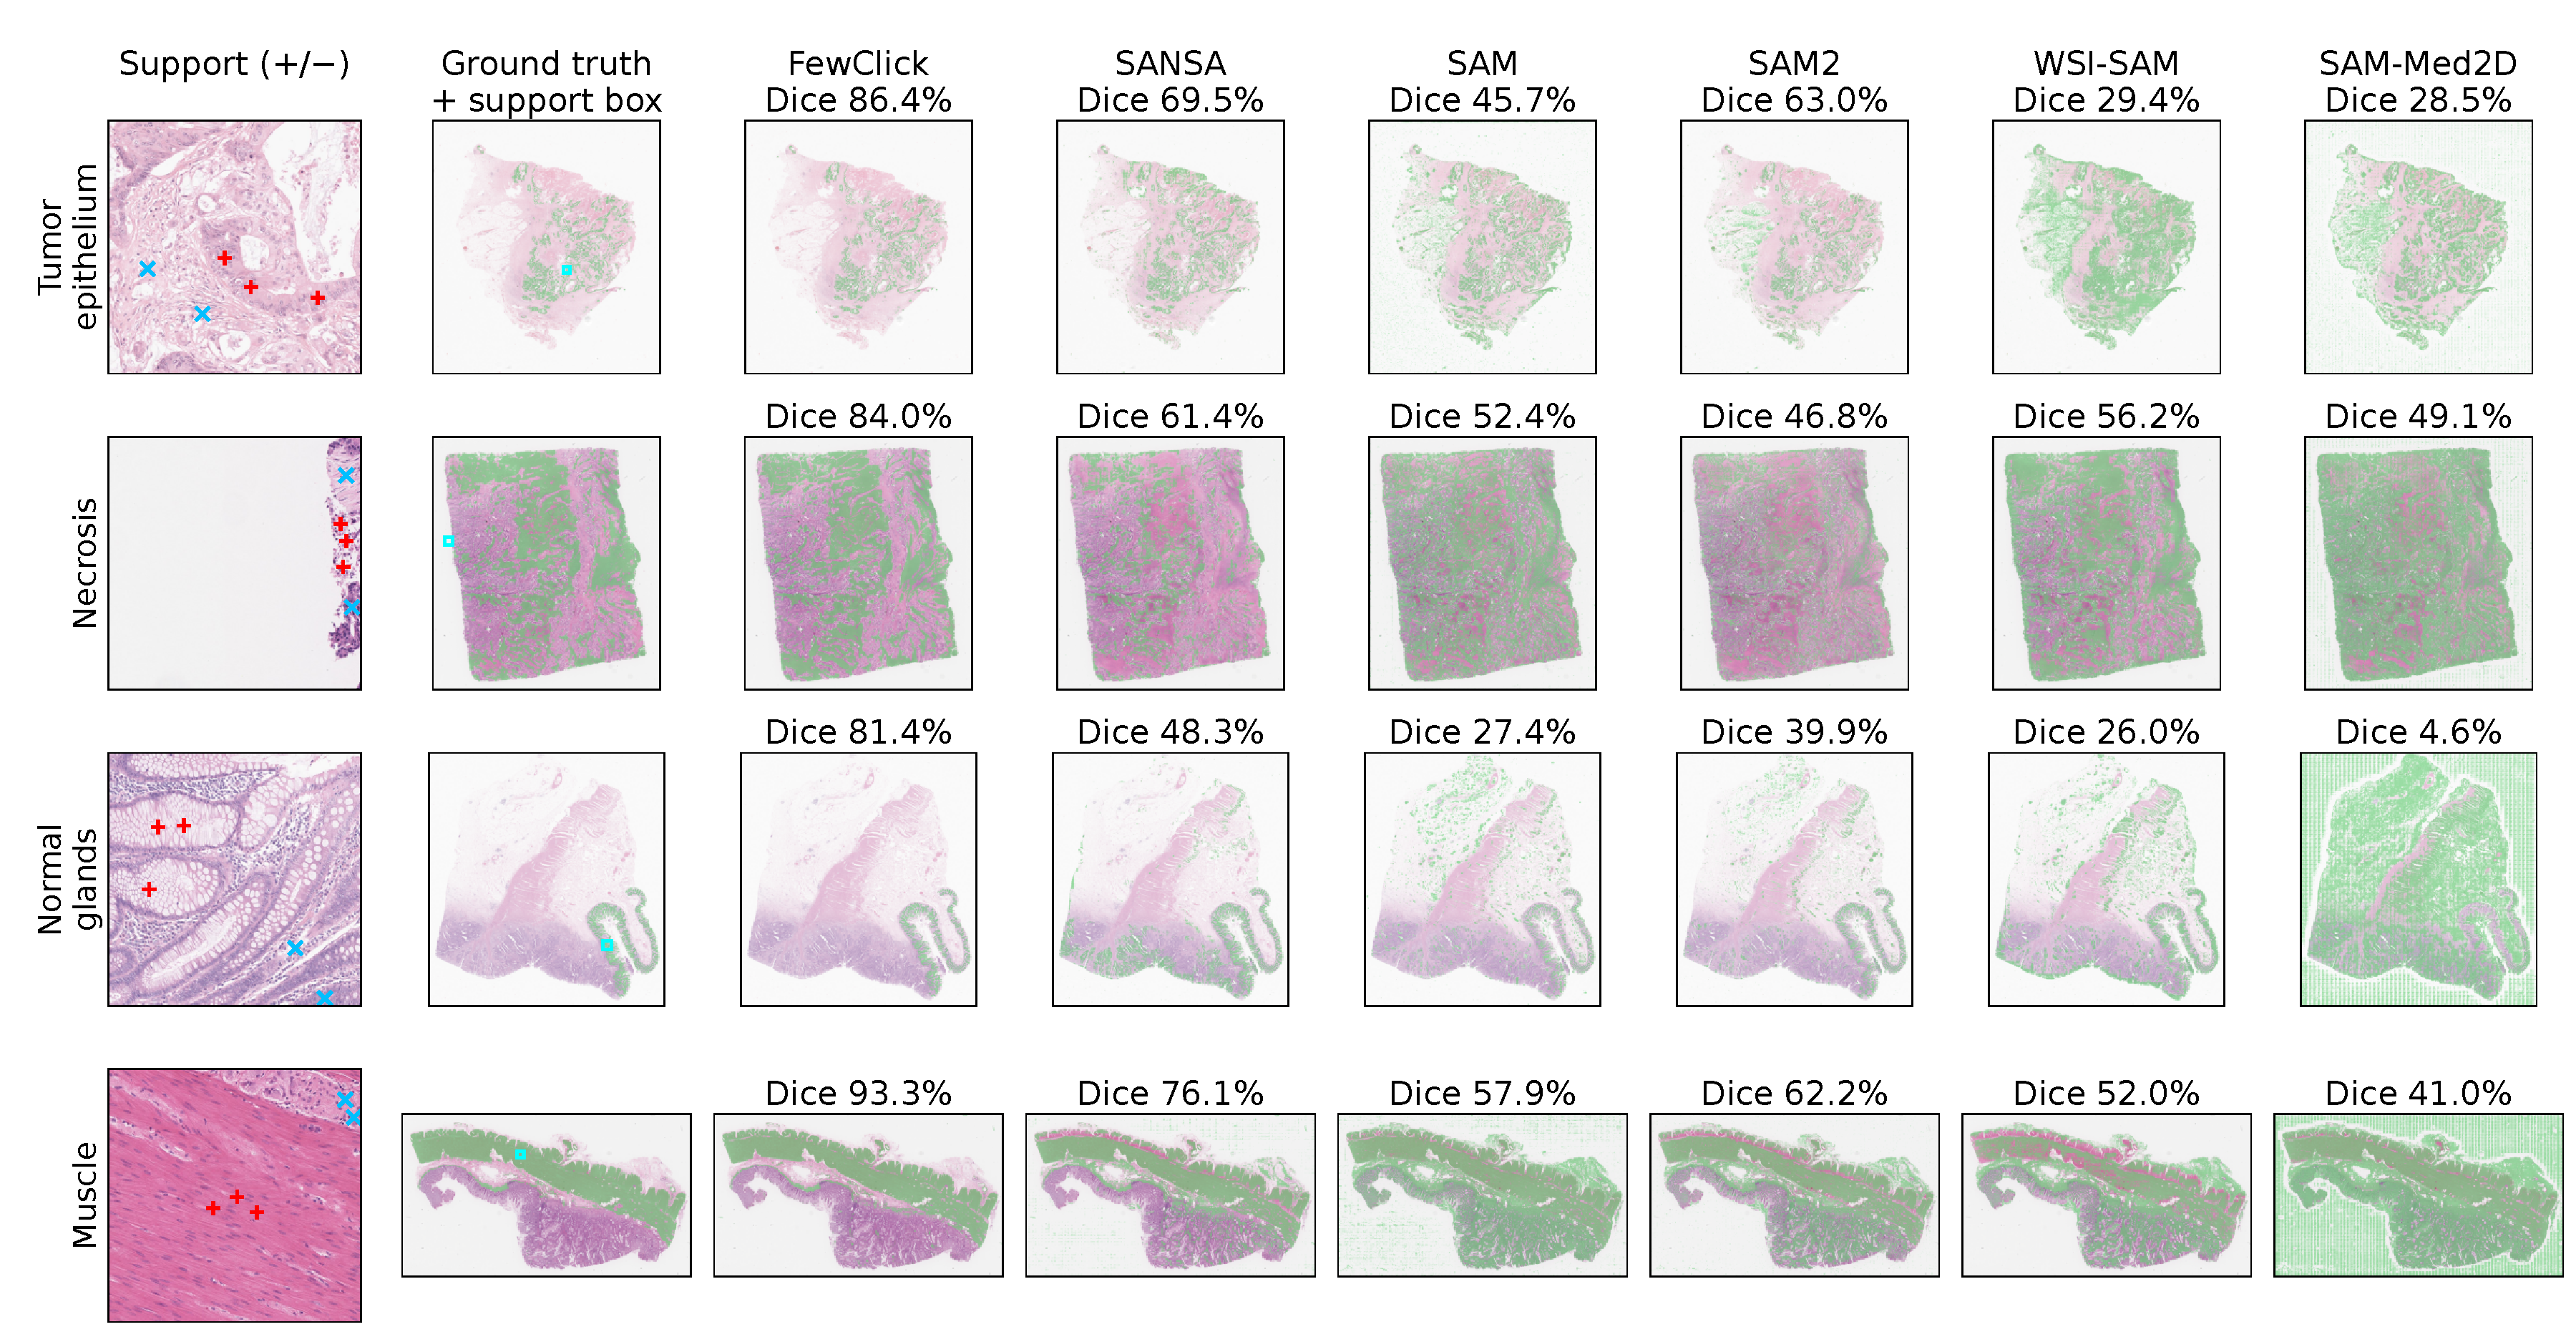
\includegraphics[width=\textwidth]{figures/figure2.pdf}
\caption{选取的整片分割案例，每个案例使用一个支持集。各行依次为肿瘤上皮、坏死、正常腺体和肌层；各列为支持点击、带支持框的真实标注及六种方法的预测。红色加号与天蓝色叉号分别表示正负点击。绿色覆盖表示目标组织，青色框标示支持图像块。面板分数为相应“切片—目标”组合的整片Dice，基于原始分辨率的有效像素计算。}
\label{fig:wsi}
\end{figure*}
六种方法在15张WSI上完成了912次“组织—方法”评价。FewClick的整片宏平均Dice为43.75\%，严格远端宏平均Dice为40.98\%，分别比SANSA的33.23\%与30.12\%高10.52和10.86个百分点（表~\ref{tab:wsi}）。排除输入覆盖范围与支持区域相交的相关输出后，增益仍然存在。对每张切片内可评价的组织取平均后，FewClick在两个评分域上均优于SANSA，覆盖15张切片中的14张。以切片为聚类单位的配对Bootstrap给出整片与严格远端增益的95\%置信区间，分别为$[7.62,13.56]$和$[8.02,13.87]$个百分点。

在11种组织中的10种上，FewClick的整片Dice高于SANSA；脂肪组织略低。正常腺体与淋巴组织聚集分别提高17.13和28.78个百分点（表~\ref{tab:wsi_tissue}）。二者在严格远端域上的增益仍为18.04和29.11个百分点，支持了超出支持邻域的迁移能力。图~\ref{fig:wsi}展示了选取的组织案例。

\paragraph{从窗口到整张切片。}
在正式评价的前三张WSI上（32个“切片—目标”组合），FewClick与SANSA的目标存在窗口Dice分别为37.79\%和37.37\%；融合后的整片Dice为45.65/34.85\%。将每个像素分配给覆盖它且中心最近的窗口，不进行重叠平均时，整片Dice为46.41/34.70\%。因此，整片增益在重叠平均之前就已存在。目标存在窗口Dice仅对含有目标的窗口取平均，而整片Dice对每个有效像素计数一次，并包含目标缺失窗口中的误报。在这些窗口中，FewClick/SANSA的FPA为3.26/8.31\%。较低的目标缺失窗口FPA有助于形成更大的整片增益；该指标同时反映目标覆盖与对非目标区域的排除。

\begin{figure*}[t]
\centering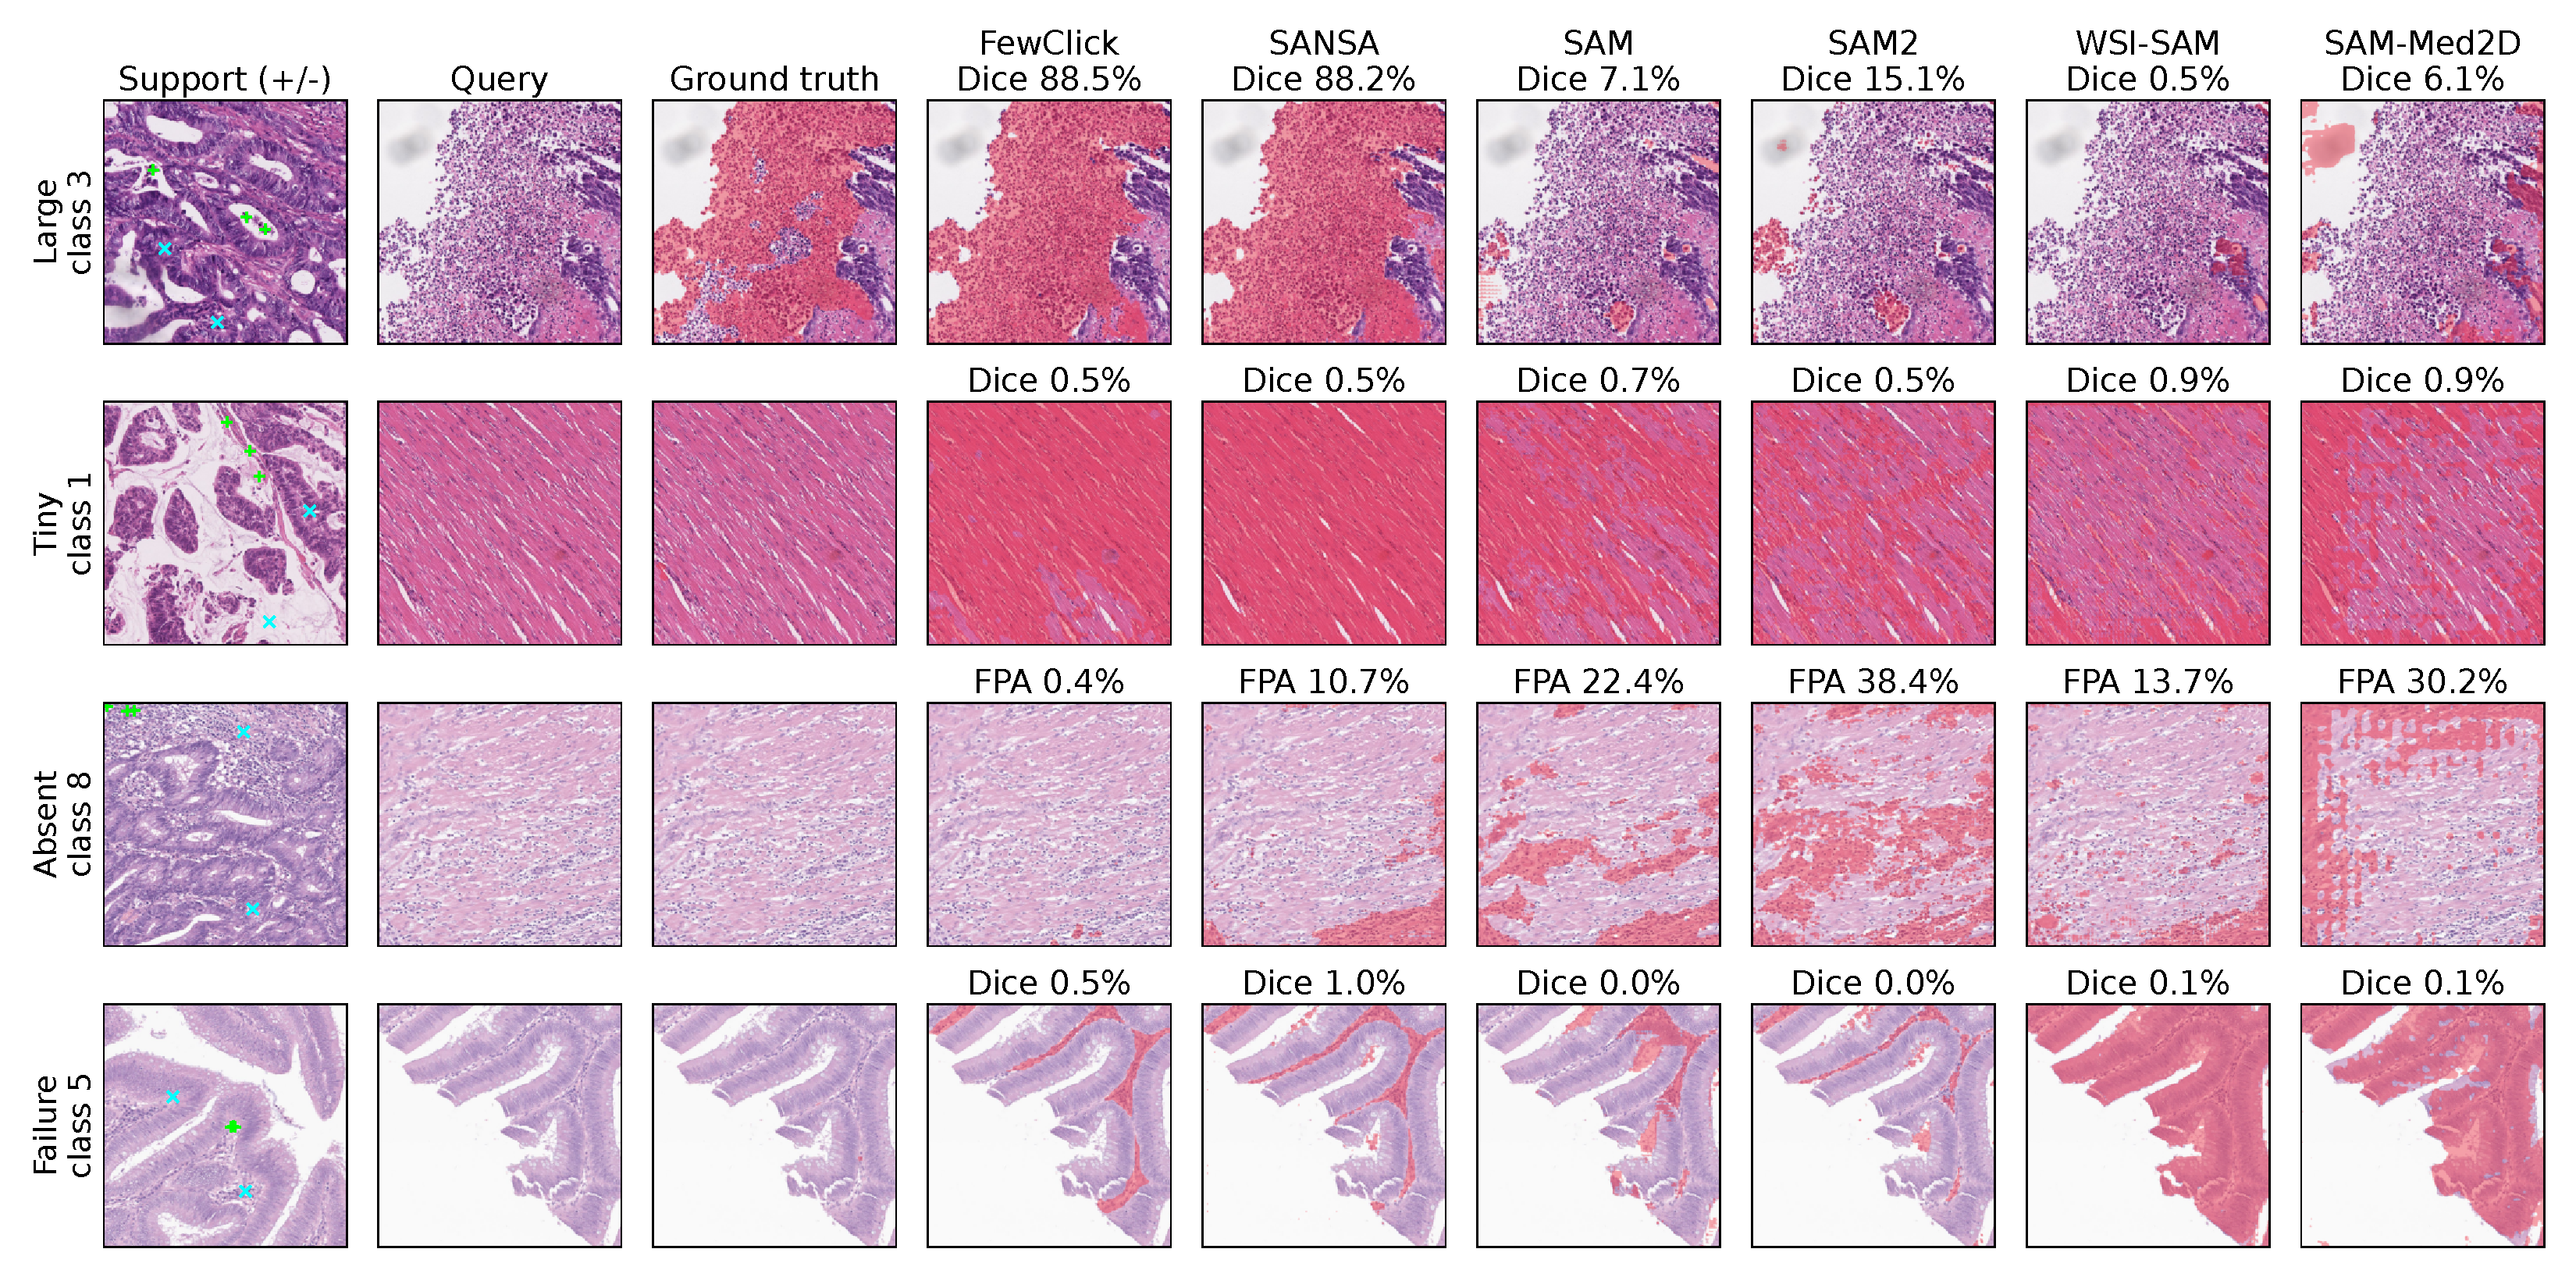
\includegraphics[width=\textwidth]{figures/figure3.pdf}
\caption{远端定性案例：大目标、微小目标、目标缺失及低Dice失败案例。每行包含支持点击、查询图像、真实标注及六种方法的预测。案例选取各组中最接近FewClick Dice中位数（目标存在）或FPA中位数（目标缺失）的任务，并以任务索引打破并列。绿色加号与青色叉号分别表示正负支持点击；红色覆盖表示目标组织。目标存在案例的面板分数为任务级Dice，目标缺失案例为FPA。指标基于原始$512\times512$预测计算。}
\label{fig:failures}
\end{figure*}

\subsection{结构消融}
\begin{table}[t]
\centering
\caption{匹配条件下的结构消融：(a) 精细表征与密集迁移；(b) 融合模型的组件。P/L/S分别表示目标存在、大目标和小目标Dice；所有数值均为百分比。Dice越高越好，FPA越低越好。}
\label{tab:ablation}
\small
\setlength{\tabcolsep}{4pt}
\textbf{(a) 精细表征 $\times$ 密集迁移}\\[2pt]
\begin{tabular}{@{}llrrr@{}}
\toprule
精细视野 & 迁移 & P & L & FPA \\
\midrule
整块 & 否 & 39.19 & 73.81 & 6.71 \\
整块 & 是 & 39.97 & 76.51 & 8.10 \\
分块 & 否 & 40.16 & 74.63 & 5.74 \\
分块 & 是 & 40.87 & 76.84 & 7.04 \\
融合 & 否 & 40.92 & 75.37 & 5.61 \\
融合 & 是 & 42.11 & 78.49 & 7.75 \\
\bottomrule
\end{tabular}
\par\vspace{4pt}
\textbf{(b) 融合模型组件}\\[2pt]
\begin{tabular}{@{}lrrrr@{}}
\toprule
变体 & P & L & S & FPA \\
\midrule
完整FewClick & 42.11 & 78.49 & 28.19 & 7.75 \\
无密集迁移 & 40.92 & 75.37 & 28.04 & 5.61 \\
无区域消息 & 41.66 & 77.66 & 28.09 & 6.90 \\
\bottomrule
\end{tabular}
\end{table}

我们在使用与不使用密集迁移两种条件下，分别训练整块、四分块和等权融合表征，形成$2\times3$组比较。各模型均从相同的公开初始化出发，遵循$9{,}500$个任务／$2{,}375$次更新的预算，并在相同的$11{,}000$个远端任务上评价。

\paragraph{同特征原型基线。}
Proto-MS使用轻量卷积解码器，根据正负点击原型与相似度预测掩码。它与FewClick共享冻结的Phikon-v2、三个物理视野、整块／分块等权融合、七次编码及训练预算。共同子集包含550个小目标、262个大目标及275个目标缺失任务，抽样不使用模型预测。目标存在Dice按各组织在原队列中的大小目标比例加权。在这$1{,}087$个任务上，FewClick的目标存在Dice提高1.49个百分点（42.32\%对40.83\%），大目标Dice提高4.17个百分点（75.67\%对71.50\%）。其目标缺失FPA更高，为6.32\%，Proto-MS为5.16\%。在三张WSI上，融合后的整片Dice从Proto-MS的42.13\%提高至FewClick的45.65\%。这些分割重叠增益在相同预训练特征和输入视野下仍然存在。

\paragraph{密集概率迁移。}
在融合特征下，加入密集迁移使目标存在Dice从40.92\%提高至42.11\%，大目标Dice从75.37\%提高至78.49\%；根据未舍入数值计算的增益分别为1.20和3.13个百分点。小目标Dice从28.04\%提高至28.19\%。FPA从5.61\%上升至7.75\%，说明该组件主要改善较大的目标区域，同时增加了目标缺失时的响应。

\paragraph{整块与分块表征。}
无论是否使用密集迁移，融合表征均获得最高的目标存在Dice和大目标Dice（表~\ref{tab:ablation}a），支持了完整组织结构与局部细节的互补作用。

\paragraph{跨尺度区域消息。}
保持相同视野与七次骨干网络编码，将跨尺度区域消息替换为恒等映射，并移除跨尺度解码器边后，目标存在、大目标和小目标Dice分别为41.66\%、77.66\%和28.09\%，FPA为6.90\%。大目标Dice下降0.83个百分点，小于移除密集迁移后的3.13个百分点降幅。两个组件均提高了分割重叠程度，同时增加目标缺失FPA。

\paragraph{可学习区域与固定区域。}
将可学习分配替换为固定空间软网格并进行匹配重训后，在同一组$1{,}087$个任务上，目标存在Dice为42.04\%，FewClick为42.32\%。可学习分配带来的0.28个百分点增益较小；固定网格的大目标Dice略高（76.02\%对75.67\%），而可学习区域将目标缺失FPA从6.67\%降至6.32\%。

\paragraph{各组件对整片分割的影响。}
在三张WSI上，移除密集迁移使融合后的整片Dice从45.65\%降至41.70\%，移除跨尺度区域消息后则为44.27\%。严格远端Dice呈相同排序：FewClick为43.04\%，移除密集迁移后为39.42\%，移除区域消息后为41.89\%。移除密集迁移带来的更大降幅，与其对大目标图像块Dice的更大影响一致。



\subsection{效率与提示敏感性}
\begin{table}[t]
\centering
\caption{在单张RTX 5880 Ada GPU上测量100个任务得到的平均延迟和缓存大小。首次预测包含读取与编码；改变提示后的预测复用图像特征。缓存大小包括一对支持—查询特征及提示记忆。}
\label{tab:efficiency}
\small
\setlength{\tabcolsep}{4pt}
\begin{tabular}{@{}lrrr@{}}
\toprule
方法 & 首次（ms） & 更新后（ms） & 缓存（MiB） \\
\midrule
FewClick & 1539.2 & 43.0 & 16.39 \\
SANSA & 1226.3 & 39.1 & 212.38 \\
SAM & 1191.8 & 18.0 & 16.00 \\
SAM2 & 1297.9 & 16.3 & 40.00 \\
WSI-SAM & 767.9 & 36.3 & 34.00 \\
SAM-Med2D & 863.9 & 17.7 & 1.00 \\
\bottomrule
\end{tabular}
\end{table}

六种方法在同一张GPU上依次计时，每种方法预热三次后测量100个任务。首次预测包含读取与编码，使用三个正点击和两个负点击；改变提示后的预测复用图像特征，使用一个正点击和一个负点击。计时通过GPU同步进行，不包含模型加载与评分。

FewClick首次预测平均耗时1539.2\,ms，改变提示后为43.0\,ms，SANSA分别为1226.3/39.1\,ms；二者缓存大小分别为16.39和212.38\,MiB（表~\ref{tab:efficiency}）。FewClick的缓存占用减少92.3\%，同时保持43.0\,ms的提示更新耗时。在共享GPU环境下，FewClick处理每张切片的全部目标平均需要98.0分钟，包含查询读取与编码、解码、融合、评分及保存掩码的核验。

在按组织／目标大小分层哈希选出的330个任务上（220个目标存在、110个目标缺失），将提示从三个正点击、两个负点击减少至一个正点击、一个负点击后，FewClick/SANSA的Dice从53.18/52.83\%降至51.14/51.03\%。保持三个正点击时，加入第二个负点击使FewClick的FPA从9.80\%降至8.20\%。在$512\times512$支持网格上，两像素或五像素的径向扰动使Dice变化不超过0.31个百分点。

\subsection{目标大小、边界与失败分析}

在$5{,}204$个小目标任务上，FewClick的宏平均Dice为28.19\%，SANSA为27.65\%。当目标占有效面积不足1\%时，两者的Dice均低于8\%（7.68/7.59\%）。在$1$--$5\%$与$5$--$20\%$两个面积层中，FewClick/SANSA的Dice分别升至36.98/35.59\%与59.43/59.05\%。

FewClick的总体精确率为39.67\%，高于SANSA的38.21\%；召回率为67.90\%，SANSA为77.75\%；边界F1为25.86\%，SANSA为29.25\%。对于大目标，FewClick同时提高了精确率（77.69\%对76.65\%）与召回率（83.66\%对82.98\%），但边界F1较低（40.35\%对45.51\%）。其更强的大区域覆盖能力因而与较低的精细轮廓准确性并存。

图~\ref{fig:failures}展示了大目标、微小目标、目标缺失和低Dice案例。在目标缺失示例中，FewClick/SANSA的FPA为0.40/10.67\%。在目标面积占比为0.24\%时，FewClick的Dice为0.51\%，同时出现较大范围的非目标响应。
